\documentclass[12pt]{article}

\newcommand{\cnum}{\textbf{What's Cooking?}}
\newcommand{\ctitle}[3]{\title{\vspace{-0.5in}\cnum\\#2\vspace{-1ex}}}
\usepackage{enumitem}
\usepackage{amsmath}
\usepackage[usenames,dvipsnames,svgnames,table,hyperref]{xcolor}
\usepackage{titlesec}
\usepackage{graphicx}
\usepackage[hang,flushmargin,bottom]{footmisc}
\usepackage{float}
\restylefloat{table}
\graphicspath{ {figures/} }

\newlist{legal}{enumerate}{10}
\setlist[legal]{label*=\arabic*.}

\setlength{\footnotemargin}{3mm}
\setlength{\skip\footins}{0.5cm}
\setlength{\footnotesep}{0.3cm}

\renewcommand*{\theenumi}{\alph{enumi}}
\renewcommand*\labelenumi{(\theenumi)}
\renewcommand*{\theenumii}{\roman{enumii}}
\renewcommand*\labelenumii{\theenumii.}


\begin{document}
\ctitle{0}{Machine Learning Engineer Nanodegree Capstone Project}{}
\author{Albert Pan}
\date{\vspace{-2ex}November 23, 2018}
\maketitle

\section{Definition}
\subsection{Project Overview}

Food plays a major part in any culture around the world. In fact, the geographical characteristics and cultural associations of a region directly influence their cuisines. By investigating the ingredients used in various cuisines, we can gain a better understanding of the geographical and cultural landscape of different regions.

Han Su et. al.\footnote{Su, Han \& Lin, Ting-Wei \& Li, C.-T \& Shan, Man-Kwan \& Chang, Janet. (2014). Automatic recipe cuisine classification by ingredients. UbiComp 2014 - Adjunct Proceedings of the 2014 ACM International Joint Conference on Pervasive and Ubiquitous Computing. 565-570. 10.1145/2638728.2641335.} has worked on investigating if recipe cuisines could be identified by their ingredients, using data from food.com. They treated each ingredient as a feature and examined the common ingredients for each cuisine. Their study provides good insight on how to approach this project and what results we could expect to achieve.

For this project, we can use machine learning techniques to attain useful predictions with our data. This project will give me an opportunity to work with real-world datasets and to learn about the relation between ingredients and cuisines. This kind of research can be expanded to other fields of study involving text classification.

\subsection{Problem Statement}
Using the data provided by Yummly\footnote{https://www.kaggle.com/c/whats-cooking-kernels-only/data}, the challenge is to predict the cuisine of the dish from its list of ingredients. More specifically, this would be multi-class classfication problem, as we have 20 different cuisines we can predict. We can use a machine learning model that utilizes this data to predict the appropriate cuisine.
\newline
\newline
%
My strategy for solving this problem is as follows:
\begin{enumerate}[label*=\arabic*.]
\item Download data from Kaggle
\item Explore data with visualizations
\item Preprocess data and extract features
\item Train and test model
\item Tune hyperparameters
\end{enumerate}

\subsection{Metrics}
As previously mentioned, our training data seems to be unbalanced, and thus I will be using the $F_1$-score to evaluate the model. The $F_1$-score is the weighted average of the precision and recall, and can be expressed mathematically with the following form:

\begin{equation}
F_1 = 2 \cdot \frac{precision \cdot recall}{precision+recall}
\end{equation}
%
We can also take a look at the precision and recall metrics on their own. Precision can be expressed with the following equation, where $dish_x$ is a dish of a particular cuisine $x$:

\begin{equation}
precision = \frac{\textit{$dish_x\: correct$}}{\textit{$total\: dish_x$}}
\end{equation}
%
where $dish_x\: correct$ is the number of dishes of cuisine $x$ that are correctly classified as $x$, and $total\: dish_x$ is the the total number of dishes that were classified as $x$.
\newline
\newline
%
Recall can expressed with:

\begin{equation}
recall = \frac{\textit{$dish_x\: correct$}}{\textit{$dish_x\: correct$} + \textit{$dish_x\: incorrect$}}
\end{equation}
%
where $dish_x\: correct$ is the number of dishes of cuisine $x$ that are correctly classified as $x$, and $dish_x\: incorrect$ is the number of dishes of cuisine $x$ that are incorrectly classified.

\section{Analysis}
\subsection{Data Exploration}
The dataset that I will be using is provided by Yummly, and it consists of two JSON files. The most important file is the \textit{train.json} file, which has 39774 rows of data, and this is the data that I will be using to train the model. The \textit{test.json} file has 9944 rows of data, and this is the data that I will be using to evaluate the model.

\begin{table}[H]
\centering
\begin{tabular}{|l|l|l|}
\hline
\textbf{id} & \textbf{cuisine} & \textbf{ingredients}                                     \\ \hline
10259       & greek            & {[}romaine lettuce, black olives, grape tomatoes, ...{]} \\ \hline
22213       & indian           & {[}water, vegetable oil, wheat, salt{]}                  \\ \hline
12734       & italian          & {[}chopped tomatoes, fresh basil, garlic, ...{]}         \\ \hline
41995       & mexican          & {[}ground cinnamon, fresh cilantro, chili powder, ...{]} \\ \hline
2941        & thai             & {[}sugar, hot chili, asian fish sauce, lime juice{]}     \\ \hline
\end{tabular}
\caption{A few examples from our training dataset.}
\end{table}

\noindent
The training data contains three fields, \textit{id}, \textit{cuisine}, and \textit{ingredients}. The \textit{id} field is a unique integer identifier for a particular dish, and is not needed for modeling or analysis. The other two fields, \textit{cuisine} and \textit{ingredients}  are very important. \textit{ingredients} consists of the list of ingredients for each dish, while \textit{cuisine} denotes the cuisine. I will be extracting the features from \textit{ingredients} and I will be trying to predict the target class \textit{cuisine}.

\subsection{Exploratory Visualization}

To better understand the data, we can take a look at the distribution of cuisines in our training data:

\begin{figure}[!h]
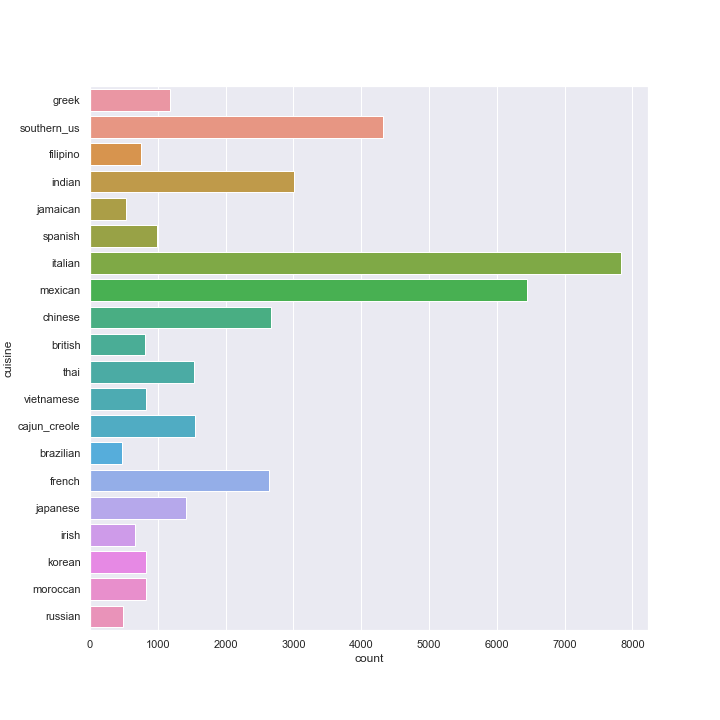
\includegraphics[width=\textwidth, height=15cm]{cuisine-distribution.png}
\caption{Cuisine distribution in training dataset}
\end{figure}

\noindent
We see that our training data is unbalanced, as there are much more "italian" and "mexican" cuisines that any of the other cuisines. This is why I decided to use the $F_1$-score as the evaluation metric, as the $F_1$-score will take into account both precision and recall.

We can also take a closer look at our ingredients. There are 6714 kinds of distinct ingredients, and there are a few ingredients in particular that are more common than the rest:

\begin{figure}[!h]
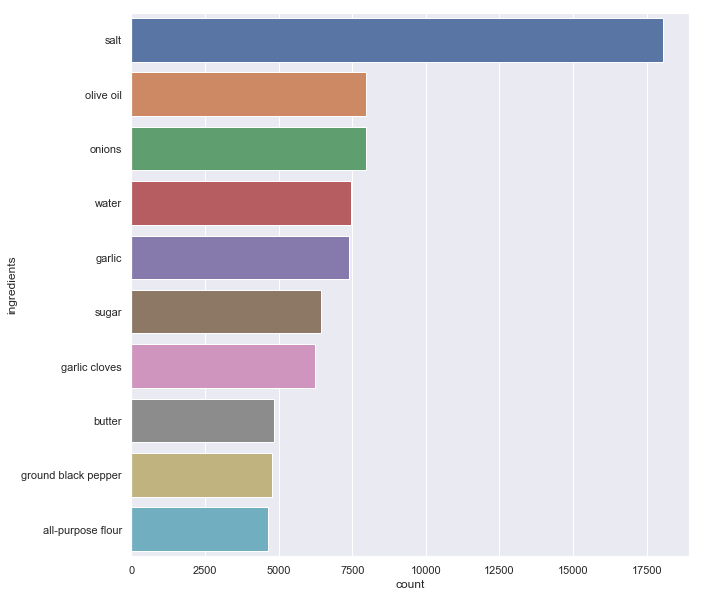
\includegraphics[width=\textwidth, height=10cm]{10-most-common-ingredients.png}
\caption{10 most common ingredients}
\label{fig:common-ingredients}
\end{figure}

We can see that a good number of ingredients are common to many different recipes and cuisines. In particular, ingredients such as \textit{salt}, \textit{olive oil}, \textit{onions}, and \textit{water} are very common, and this makes sense. \textit{Salt} is one of the ingredients that improves the flavor of a recipe, \textit{olive oil} allows for a better transfer of heat for cooking, and so on. All of the ingredients shown in Figure \ref{fig:common-ingredients} are essential to cooking, and it really captures the ingredients that most cuisines have in their dishes.

One important point to mention is that some ingredients are very similar to each other in both name and in usage. For example, let's take a look at \textit{garlic} and \textit{garlic cloves}. They are both \textit{garlic} ingredients, and mainly serve the same purpose in a dish. Other examples include \textit{eggs} and \textit{large eggs}, as well as \textit{ground black pepper} and \textit{black pepper}. Thus, I will combine these ingredients into one homogenous ingredient.

Since the ingredients mentioned above are common to many cuisines, they may not be very helpful for distinguishing one cuisine from another. We can filter out the most common ingredients from the ingredients used in \textit{Italian} and \textit{Mexican} dishes and see what they tell us:

\begin{figure}
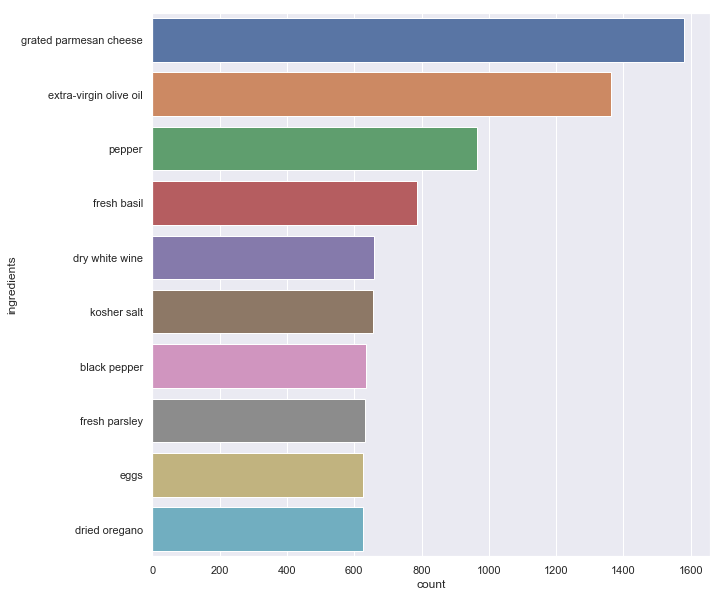
\includegraphics[width=\textwidth, height=10cm]{italian-most-common-ingredients.png}
\caption{Italian 10 most common ingredients}
\label{fig: italian-most-common-ingredients}
\end{figure}

\begin{figure}
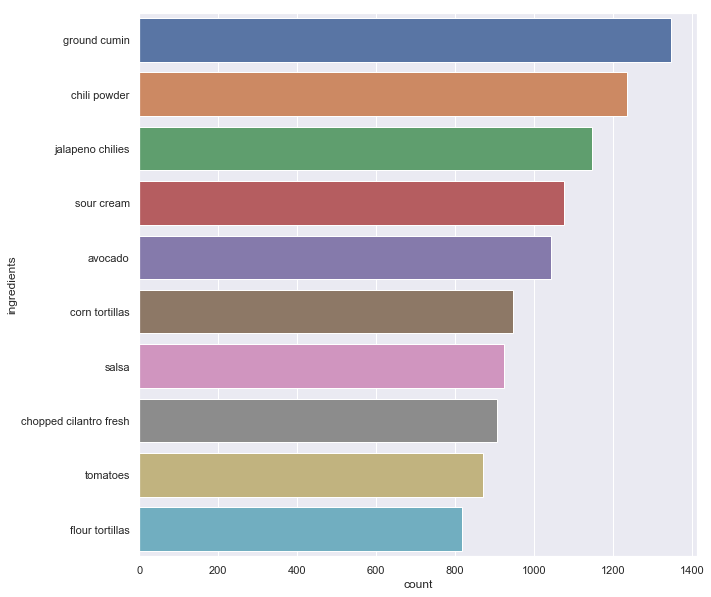
\includegraphics[width=\textwidth, height=10cm]{mexican-most-common-ingredients.png}
\caption{Mexican 10 most common ingredients}
\label{fig: mexican-most-common-ingredients}
\end{figure}

Once I filtered out the most common ingredients, we can see the ingredients that are representative of their respective cuisines, as evidenced in figures \ref{fig: italian-most-common-ingredients} and \ref{fig: mexican-most-common-ingredients}. These are the ingredients that will distinguish a certain cuisine from another cuisine, and we will be focusing on extracting these ingredients in our data preprocessing.

\subsection{Algorithms and Techniques}
This is a classification problem, and so I will be using algorithms and techniques that are suited for classification problems. In particular, I will be using the following models/algorithms:

\begin{itemize}
	\item Support Vector Machines (LinearSVC\footnote{https://scikit-learn.org/stable/modules/generated/sklearn.svm.SVC.html}): Support vector machines, or SVMs, are a set of supervised learning models that uses decision boundaries for both classification and regressions problems. SVMs construct a hyperplane that allows us to linearly separate data by transforming the feature space. For this problem, I decided to use a linear kernel because it is less computationally expensive and allows us to use multi-class classification.
	\item Naive Bayes (MultinomialNB\footnote{https://scikit-learn.org/stable/modules/generated/sklearn.naive\_bayes.MultinomialNB.html}): Naive Bayes is a supervised learning algorithm that is based on Bayes' Theorem\footnote{https://en.wikipedia.org/wiki/Bayes\%27\_theorem}, and it assumes that all of the features are independent. This particular algorithm has been historically used for SPAM detection for its speed and accuracy. For this problem, I will be using MultinomialNB (Multinomial Naive Bayes model), which is a multi-class classifier implementation of Naive Bayes.
	\item Decision Trees (DecisionTreeClassifier\footnote{https://scikit-learn.org/stable/modules/generated/sklearn.tree.DecisionTreeClassifier.html}): Decision Trees learn decision rules and generates trees that can be used for both classification and regression problems. Using the input features, it can decide which subtree to follow until it reaches the bottom of the tree, in which it will return its prediction. I will be using the DecisionTreeClassifier from the \textit{scikit-learn} library to perform multi-class classification.
	\item Random Forests (RandomForestClassifier\footnote{https://scikit-learn.org/stable/modules/generated/sklearn.ensemble.RandomForestClassifier.html}): Random forests are ensemble methods that can used to build models for classification and regression models\footnote{https://en.wikipedia.org/wiki/Random\_forest}. They operate by constructing a series of decision trees and outputting a combined prediction from all of the trees. Random Forests aim to correct the decision tree's tendency to overfit to the training data. I will be using the RandomForestClassifier, which is capable of multi-class classification.
	\item Gradient Boosted Trees (XGBClassifier \footnote{https://xgboost.readthedocs.io/en/latest/python/python\_api.html}): Gradient boosting is a technique used in both classification and regression problems. and it builds a prediction model by creating an ensemble of weak learners, usually with decision trees\footnote{https://xgboost.readthedocs.io/en/latest/tutorials/model.html}. It builds the model by utilizing the optimization of an arbitrary differentiable loss function. I will be using XGBClassifier from the \textit{xgboost} library.
\end{itemize}

\subsection{Benchmark}
For our baseline benchmark, we can use the metric obtained by predicting the most common cuisine in the training and testing datasets. The most common cuisine is \textit{Italian}, and our benchmark model will predict Italian to all recipes. This would give us a benchmark $F_1$-score of $0.3292$.

\section{Methodology}
\subsection{Data Preprocessing}
Our training dataset is divided into \textit{ingredients} and \textit{cuisine}. \textit{cuisine} is already ready for implementation. What we do have to do is preprocess each recipe's ingredients and uniformly format them. I will perform the following steps to preprocess the data:

\begin{legal}
	\item Remove non-letter characters (punctuation) using regular expressions.
	\item Convert all letters to lowercase.
	\item Remove descriptor words (e.g. chopped, minced, toasted, etc.) and combined similar ingredients into homogenous groups.
	\item Apply a lemmatization process to the words.	
	\item Convert words to vectors using tf-idf.
\end{legal}

\noindent
Lemmatization refers to the process of grouping together different inflected forms of words so that they can be analyzed as a single term\footnote{https://en.wikipedia.org/wiki/Lemmatisation}. This means that words such as \textit{tomatoes} will be transformed into \textit{tomato}, thus allowing us to treat them as the same term. I used \textit{nltk}'s WordNetLemmatizer\footnote{https://www.nltk.org/\_modules/nltk/stem/wordnet.html} to perform lemmatization on our ingredients.

tf-idf is a method in which you can extract information from a string. It evaluates the weight of the value of words according to the number of times that it appears in a text and offsets it by the number of times it appears in the entire corpus. In our problem, tf-idf seems to work well because the number of times an ingredient appears in the recipe of a particular cuisine could help us determine if that specific ingredient is indicative to that cuisine. We will use the output of \textit{scikit-learn}'s TfidfVectorizer\footnote{https://scikit-learn.org/stable/modules/generated/sklearn.feature\_extraction.text.TfidfVectorizer.html} to obtain the count matrix that we will use as input for our model.

I will also convert our \textit{cuisine} class to integer representation using \textit{scikit-learn}'s label encoder\footnote{https://scikit-learn.org/stable/modules/generated/sklearn.preprocessing.LabelEncoder.html} so that the model can recognize our target class.

\subsection{Implementation}
I did not change the evaluation metric ($F_1$-score), as it works well in our case since we have an uneven distribution of data.

The supervised learning algorithms that we used were initialized with the default parameters. All of the models are from the \textit{scikit-learn} library, with the exception of the XGBClassifier, which is from the \textit{xgboost} library.

The test data can only be evaluated on the Kaggle competition, and so we split our training data into 70\% training and 30\% testing.

\subsection{Refinement}

I trained all of the models and got their training and testing scores. To refine the models, I tuned their hyper-parameters using \textit{scikit-learn}'s GridSearchCV\footnote{https://scikit-learn.org/stable/modules/generated/sklearn.model\_selection.GridSearchCV.html}. GridSearchCV allows us to perform an exhaustive search over all the hyper-parameters that we specify in a 5-fold cross-validated dataset. I then used the optimized classifier and re-evaluated its performance.

\section{Results}
\subsection{Model Evaluation and Validation}
After training and testing all the models, I have plotted the results in the figure below:

\begin{figure}[!h]
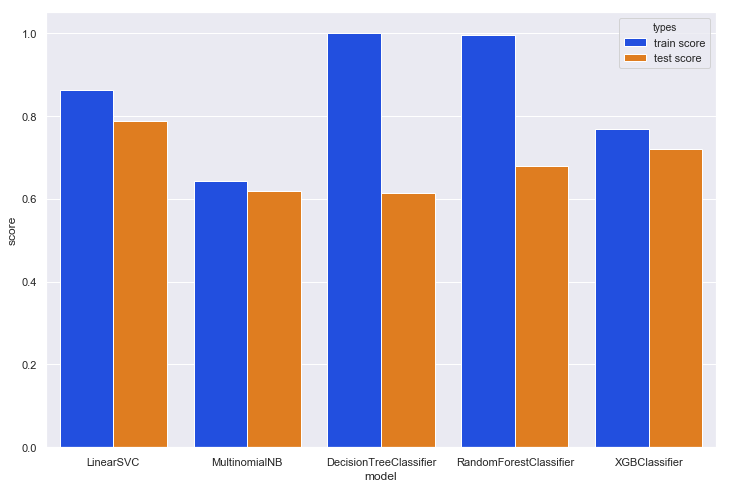
\includegraphics[width=\textwidth, height=10cm]{results.png}
\caption{Train and Test Score of Models}
\label{fig: model-results}
\end{figure}

\noindent
As evidenced by the figure above, we can see that the LinearSVC and the XGBClassifier perform the best, as their test scores are the two highest. The DecisionTreeClassifier and the RandomForestClassifier both have training scores that are almost 1, but have test scores that are low in comparison to the other models. This tells us that the DecisionTreeClassifier and the RandomForestClassifier are most likely overfitting to the data, which results in a low test score.

The MultinomialNB model has the worst training score and testing score out of all the models that we used. This is surprising given that Naive Bayes is usually used for  text processing. I suspect that we cannot assume that the features (ingredients) are independent, and thus it is difficult for the Naive Bayes algorithm to perform correctly. It's also possible that we have too many features that are varied from each other.

To decide which model I wanted to refine, I took a look at the training time of each of the models:

\begin{figure}[!h]
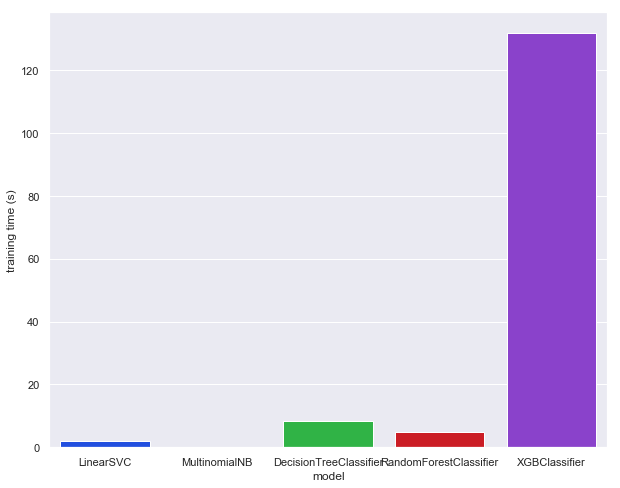
\includegraphics[width=\textwidth, height=10cm]{training_times.png}
\caption{Training Times of the Models}
\label{fig: training-times}
\end{figure}

\noindent
Between the LinearSVC and the XGBClassifier, it is clear that the LinearSVC has the XGBClassifier beat in both the test scores and the training times, as the LinearSVC is over 120x faster than the XGBClassifier. 

To tune the parameters of the LinearSVC, I chose the following two parameters: the $C$ parameter and the $max\_iterations$ parameter. The $C$ parameter represents the penalty for misclassifying a dish. Higher values of C will make the model more granular and penalize a lot for any misclassification. Given that there are only 20 cuisine classes in our dataset, I specifically chose values of C that were below $1$. The lower values will allow the model to have a larger margin of error, but it will also allow the model to learn from its mistakes and consequently improve the score. As for the $max\_iterations$ parameter, I wanted to allow the model the freedom to train for more iterations and potentially improve its scores without overfitting, and thus I selected values from the range $500-10000$.

The optimized parameters are shown in the table below:

\begin{table}[H]
\centering
\begin{tabular}{|l|l|l|l|l|l|l|}
\hline
\textbf{C}               & 0.001        & 0.01 & 0.05 & 0.1  & \textbf{0.5} & 1 \\ \hline
\textbf{max\_iterations} & \textbf{500} & 1000 & 2000 & 5000 & 10000        &   \\ \hline
\end{tabular}
\caption{Optimized values obtained from GridSearchCV}
\end{table}

\noindent
The best estimator had the parameter values of $C=0.5$ and $max\_iterations=500$. This slightly improved our testing score from $0.78639$ to  $0.78660$. It seems that our original model had parameters that were close to the optimal values already.

I then used my optimized model to predict the cuisines of the dishes in the \textit{test.json} file, and I submitted the predictions to the Kaggle competition. My model got a score of $0.78571$, which I believe is the accuracy score. 

\begin{figure}[!h]
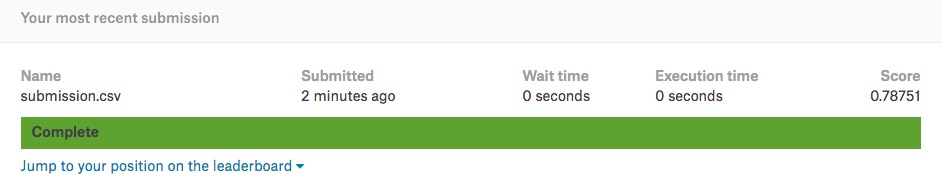
\includegraphics[width=15 cm, height=3cm]{kaggle-submission-rank.JPG}
\caption{Kaggle Competition Score}
\label{fig: kaggle-score}
\end{figure}

While I am unable to see my place on the public leaderboard, I was able to examine the leaderboards manually and I saw that my score of $0.78571$ would rank $307$ on the public leaderboard.

\begin{figure}[!h]
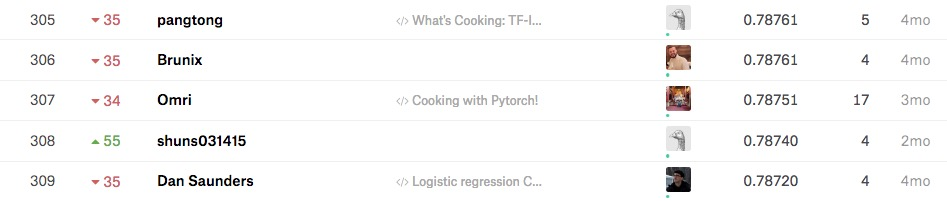
\includegraphics[width=14cm, height=3cm]{rank-comparison.JPG}
\caption{Rank on Kaggle Leaderboard}
\label{fig: kaggle-rank}
\end{figure}

\subsection{Justification}

The final result is excellent in comparison to our benchmark score of $0.3292$. I was able to achieve a $F_1$-score of $0.786$ while minimizing the training time of the model. Our model can be a solution to our problem because misclassifying a recipe would not cause any major disaster. I think that Yummly should feel confident in using my model to recommend/label dishes with a certain cuisine.

\section{Conclusion}
\subsection{Free-Form Visualization}

From Figure \ref{fig: common-ingredients-comparison}, we can see that the importance of properly cleaning and preprocessing the data. In this problem, I removed the unwanted descriptor words from the ingredients and combined the remaining terms into one homogenous group when appropriate. For example, the first graph shows both \textit{garlic} and \textit{garlic cloves} in the top 10 common ingredients, while the second graph only shows \textit{garlic}. In the second graph, \textit{garlic} is a group that represents the \textit{garlic} ingredient, so it encompasses \textit{garlic cloves} and \textit{garlic} into one group, \textit{garlic}. One thing to note is that this kind of preprocessing could diminish the importance of some ingredients, such as \textit{crushed red peppers} and \textit{red peppers}. There could be a fundamental difference in the way these two ingredients are used, so this is something we should be aware of.

When working with real-world datasets, data preprocessing is one of the most important aspects that is often overlooked. Without proper data preprocessing, the data that we have would be useless. According to a study done in 2017, data scientists spend ``80\% of their time preprocessing the data and 20\% of their time doing actual data analysis\footnote{https://www.infoworld.com/article/3228245/data-science/the-80-20-data-science-dilemma.html}". Thus, we need to make sure that we are carefully cleaning our data for our model to function properly.

\begin{figure}[H]
\centering
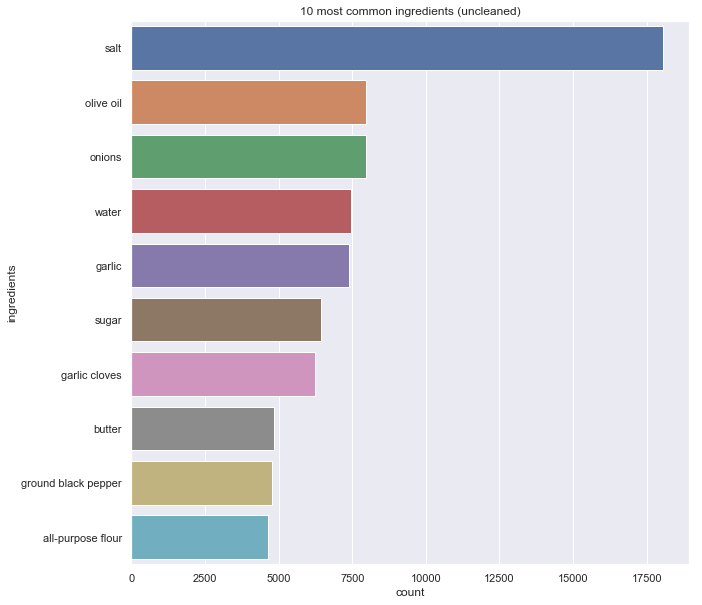
\includegraphics[width=13cm, height=9.5cm]{10-most-common-ingredients-uncleaned.png}
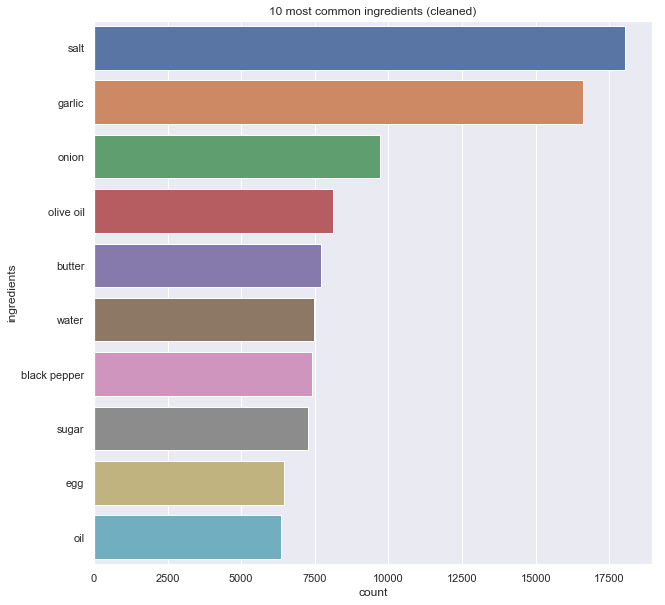
\includegraphics[width=13cm, height=9.5cm]{10-most-common-ingredients-cleaned.png}
\caption{Comparison between the most common ingredients uncleaned vs. cleaned}
\label{fig: common-ingredients-comparison}
\end{figure}

\subsection{Reflection}

I really enjoyed working on this project because it gave me a chance to work with real-world data, which was very messy. I spent a good portion of time figuring out the best way to clean the data, and I'm very satisfied with the results of my model. I also got a chance to use different libraries such as nltk and xgboost, and it was really fun figuring out how to properly implement them into this project.

From this project, I was able to better understand the process that goes into creating a machine learning model. You have to visualize and understand what's in your dataset before you're able to start preprocessing it. In fact, visualizing your dataset is a great way to find any patterns or outliers that you may want to take care of. Once you finish preprocessing your data, you need to select an appropriate model that fits your problem. Then you train and evaluate your models, and you select whichever model performs the best. From there, you can optimize your chosen model and try to improve its performance.

\subsection{Improvement}

There are definitely many improvements I can make to this project. First of all, this model could be improved if we had an even larger dataset. Some of the cuisines did not have that many dishes, and thus the model may not have to classify those cuisines very well.

Another improvement I could have made is classifying ingredients into categories such as \textit{sweet}, \textit{salty}, \textit{sour}, etc. This would greatly help the model identify foods such as desserts (sweet ingredients), and thus the model can learn to associate dishes that contain sweet ingredients with cuisines that may have more desserts than others.

I would have also liked to try using some deep learning models. Deep learning models can be used in text analysis, and given the proper computing power, a deep learning model could potentially identify stronger relationships between certain ingredients and cuisines.

All in all, I think my model does a good job of associating the ingredients to the proper cuisine. I believe there are better solutions to this problem (as mentioned above), and I think that my model can be used a good benchmark for future models.

\end{document}
